\documentclass[11pt]{article}
\usepackage[a4paper,left=10mm,right=10mm,top=15mm,bottom=15mm]{geometry}
\usepackage{amsmath,amsfonts,amsthm}
\usepackage{booktabs,float,multirow}
\usepackage{cancel}
\usepackage{graphicx}
\usepackage{hyperref}
\hypersetup{
    colorlinks=true, %set true if you want colored links
    linkcolor=blue,
    linktoc=all, %set to all if you want both sections and subsections linked
    citecolor=black,
    filecolor=black,
    urlcolor=black
}
\usepackage[UTF8]{ctex}

\newcommand{\E}{\operatorname{E}}
\newcommand{\Cov}{\operatorname{Cov}}
\newcommand{\Var}{\operatorname{Var}}

\newtheorem{theorem}{Theorem}[section]
\newtheorem{lemma}[theorem]{Lemma}

\title{BSM公式}
\author{杨弘毅}
\date{创建: 2020 年 4 月 19 日 \\修改: \today}

\begin{document}
\maketitle

\tableofcontents

\section{布朗运动、维纳过程}

标准布朗运动简易表达式(连续形式)有,其中$\varepsilon \sim N(0,1)$:
\begin{equation*}
    dZ_t = \varepsilon_t \sqrt{dt}
\end{equation*}

离散形式有:
\begin{equation*}
    Z_T - Z_t = \sum^n_{i=1} \varepsilon_i \sqrt{\Delta t}
\end{equation*}

\subsection{特征}
\textbf{标准布朗运动(Brownian motion)或维纳过程(Wiener process)}的特征有:
\begin{itemize}
    \setlength{\itemsep}{0em}
    \item 初值为零
    \item 连续
    \item 独立增量:对于任意两个不同时间点$\Delta t_i$与$\Delta t_j$,其增量$\Delta Z_i$与$\Delta Z_j$相互独立
    \item 独立同分布(方差可加):增量$\Delta Z$服从均值为零、方差等于时间长度的正态分布,即$\Delta Z_i  \sim N(0,\Delta t_i)$
\end{itemize}

\subsection{为何使用标准布朗运动}

\begin{itemize}
    \setlength{\itemsep}{0em}
    \item 股价不能为负,所以不能遵循正态分布,但股票连续复利收益率($d\ln S$)近似服从正态分布
    \item 维纳过程是一个马尔可夫随机过程,增量$\Delta Z$独立,与弱式EMH相同,即技术分析无效,无法使用历史信息预测未来,过去信息跟未来信息相互独立
    \item 维纳过程对时间处处不可导,且二次变分(Quadratic Variation)不为零,与股票价格变化存在转折尖点的性质相符
\end{itemize}

\subsection{部分证明}

\textbf{增量均值为零,方差为时间长度},当$X$与$Y$独立时,则有:
\begin{equation*}
    \Var(XY) = \Var(X)\Var(Y) + [\E(X)]^2 \Var(Y) + [E(Y)]^2 \Var(X)
\end{equation*}

此时,由于$\varepsilon_t$与$dt$独立,套用上式,同时由于$\varepsilon_t \sim N(0,1)$,则有:
\begin{equation*}
    \E(dZ_t) = \E(\varepsilon_t \sqrt{dt}) = 0
\end{equation*}

\begin{align*}
    \Var(dZ_t) & = \Var( \varepsilon_t \sqrt{dt}) \\
    & =  \Var(\varepsilon_t) \Var(\sqrt{dt}) + [\E(\varepsilon_t)]^2 \Var(\sqrt{dt}) + [E(\sqrt{dt})]^2 \Var(\varepsilon_t) \\
    & = \Var(\varepsilon_t) \left[ \Var[(\sqrt{dt})^2] - [\E(\sqrt{dt})]^2 \right] \\
    & = \Var(\varepsilon_t) \left[ \E[(\sqrt{dt})^2] - [\E(\sqrt{dt})]^2 + [\E(\sqrt{dt})]^2 \right] \\
    & = 1 \cdot \E(dt) = dt
\end{align*}

\textbf{方差可加性},由下式可见,由于独立增量,导致协方差项为零,使得方差可加。
\begin{align*}
     & \Var(X_1+X_2+X_3) \\
     & = \Var(X_1) + \Var(X_2) + \Var(X_3) \\
     & + \Cov(X_1,X_2) + \Cov(X_2,X_3) + \Cov(X_1,X_3)
\end{align*}

由上可知,增量在连续形式$dZ_t$以及离散形式$Z_T-Z_t$下,均服从均值为零,方差为时间长度的正态分布,即有:
\begin{align*}
    dZ_t & \sim N(0,dt) \\
    Z_T - Z_t & \sim N(0,T-t)
\end{align*}

\subsection{几种随机过程}

\textbf{广义维纳过程(generalized Wiener process)},a与b为常数。此时,易知其均值为$\E(dX_t) = adt$,由于$b$为常数,且$\Var(dZ_t)=dt$,则有方差为$\Var(dX_t)=b^2 dt$。
\begin{equation*}
    dX_t =a dt + b dZ_t
\end{equation*}

\textbf{普通布朗运动},a(t)与b(t)都是t的确定性函数。由于都为确定函数,所以如上可知,其均值方差为$\E(dX_t) = a(t)dt$,由于$b$为常数,且$\Var(dZ_t)=dt$,则有方差为$\Var(dX_t)=b(t)^2 dt$。
\begin{equation*}
    dX_t =a(t) dt + b(t) dZ_t
\end{equation*}

\textbf{扩散过程(Diffusion Process)},此时$a(X(t),t)$与$b(X(t),t)$都为$X_t$和$t$的确定性函数。由于漂移项与方差项都包含$X(t)$,使得扩散之后过程的条件分布无法保证仍是正态分布。但更能刻画一般动态变化,未加入新的风险源,仍具有独立增量,马尔可夫性,和方差可加性等性质。
\begin{equation*}
    dX_t =a(X(t),t) dt + b(X(t),t) dZ_t
\end{equation*}

\textbf{伊藤过程(Itô Process)},最一般化的随机过程,$a_t$和$b_t$为任意函数或随机过程。
\begin{equation*}
    dX_t =a_t dt + b_t dZ_t
\end{equation*}

\section{伊藤引理(Itô lemma)}

若变量$X_t$遵循伊藤过程:
\begin{equation*}
    dX_t =a_t dt + b_t dW_t
\end{equation*}

在导数$\dfrac{\partial f}{\partial t}$、$\dfrac{\partial f}{\partial X}$与$\dfrac{\partial^2 f}{\partial X^2}$存在的前提下,则有变量$X_t$和$t$的函数$f(X(t),t)$将遵循如下过程:
\begin{equation*}
    df_t = \left(\frac{\partial f}{\partial X}a_t  + \frac{\partial f}{\partial t} + \frac{1}{2}\frac{\partial^2 f}{\partial X^2} b^2_t \right)dt + \frac{\partial f}{\partial X} b_t dW_t
\end{equation*}

为方便记忆,可记为(金融随机分析第二卷 P118):
\begin{equation*}
    \boxed{
        df(X(t),t) = f_t(X(t),t)dt + f_x(X(t),t)dX(t) + \frac{1}{2}f_{xx}(X(t),t)dX(t)dX(t)
    }
\end{equation*}

或可写为更简洁的形式:
\begin{equation*}
    \boxed{
        df = f_t dt + f_x dX + \frac{1}{2}f_{xx}dXdX
    }
\end{equation*}

\subsection*{证明}

$f(X,t)$的泰勒展开式为:
\begin{equation*}
    \Delta f_t = \frac{\partial f}{\partial X} \Delta X + \frac{\partial f}{\partial t} \Delta t + \frac{1}{2} \frac{\partial^2 f}{\partial X^2}\Delta X^2  + \frac{\partial f}{\partial X \partial t}\Delta X \Delta t + \frac{1}{2} \frac{\partial^2 f}{\partial t^2} \Delta t^2 + \dots
\end{equation*}

当$\Delta t \rightarrow 0$时,$(\Delta t)^2$,认为是高阶无穷小,可忽略。而对于$\Delta X \Delta t$项有:
\begin{align*}
    \Delta X &= a\Delta t + b \varepsilon\sqrt{\Delta t} \\
    \Delta X \Delta t &= a(\Delta t)^2 + b \varepsilon(\Delta t)^{3/2}
\end{align*}

其中的$(\Delta t)^{3/2}$项,也被认为时高阶无穷小项,可忽略。同时由于$(\Delta X)^2$项中包含$\Delta t$项,因此需要保留。因此仅考虑前三项(\textbf{注意}:此与常微分不同,而在常微分中,$(\Delta X)^2$项是也是高阶无穷小项),展开得到:
\begin{align*}
    \Delta f_t & = \frac{\partial f}{\partial X} \Delta X + \frac{\partial f}{\partial t} \Delta t + \frac{1}{2} \frac{\partial^2 f}{\partial X^2}\Delta X^2 \\
    & = \frac{\partial f}{\partial X} \Delta X + \frac{\partial f}{\partial t} \Delta t + \frac{1}{2} \frac{\partial^2 f}{\partial X^2} [a\Delta t + b\varepsilon\sqrt{\Delta t}]^2 \\
    & = \frac{\partial f}{\partial X} \Delta X + \frac{\partial f}{\partial t} \Delta t + \frac{1}{2} \frac{\partial^2 f}{\partial X^2} b^2 \varepsilon^2 \Delta t
\end{align*}

对于$\varepsilon^2 \Delta t$项,由于$\varepsilon \sim N(0,1)$,因此有$\E(\varepsilon)=0$。又因$\Var(\varepsilon)=\E(\varepsilon^2)-[\E(\varepsilon)]^2=1$,得到$\E(\varepsilon^2)=1$,同时有$\E(\varepsilon^2 \Delta t) = \Delta t$。计算$\varepsilon^2 \Delta t$的方差可得:
\begin{align*}
    \Var(\varepsilon^2 \Delta t) & = \Var(\varepsilon^2) \Var(\Delta t) + [\E(\varepsilon^2)]^2 \Var(\Delta t) + [E(\Delta t)]^2 \Var(\varepsilon^2) \\
    & = \Var(\varepsilon^2) \Var(\Delta t) + 1 \cdot \Var(\Delta t) + [E(\Delta t)]^2 \Var(\varepsilon_t^2) \\
    & = \mathcal{O}(\Delta t^2)
\end{align*}

可以认为$\varepsilon^2 \Delta t$方差为高阶无穷小,其期望为$1$。因此,可认为$\varepsilon^2 \Delta t \approx \Delta t$,可将原式化简为:
\begin{equation*}
    \Delta f_t = \frac{\partial f}{\partial X} \Delta X + \frac{\partial f}{\partial t} \Delta t + \frac{1}{2} \frac{\partial^2 f}{\partial X^2} b^2 \Delta t
\end{equation*}

而连续形式为:
\begin{align*}
    df_t & = \frac{\partial f}{\partial X}  dX_t + \frac{\partial f}{\partial t} dt + \frac{1}{2} \frac{\partial^2 f}{\partial X^2} b^2 dt \\
    & = \frac{\partial f}{\partial X} (a_t dt + b_t dZ_t) + \frac{\partial f}{\partial t} dt + \frac{1}{2} \frac{\partial^2 f}{\partial X^2} b^2 dt \\
    & = \left(\frac{\partial f}{\partial X}a_t  + \frac{\partial f}{\partial t} + \frac{1}{2}\frac{\partial^2 f}{\partial X^2} b^2_t \right)dt + \frac{\partial f}{\partial X} b_t dZ_t
\end{align*}

\section{几何布朗运动}

\subsection{推导}

由于衍生品价格是标的资产价格与时间的函数,即只需要假定标的资产遵循过程,即可用伊藤引理求得其衍生品遵循过程。假设股票价格服从几何布朗运动(Geometric Brownian Motion,GBM):
\begin{equation*}
    dS_t = \mu S_t dt + \sigma S_t dZ_t
\end{equation*}

令$f_t = \ln S_t$,此时:
\begin{equation*}
    \frac{\partial f}{\partial S} = \frac{1}{S_t}, \quad
    \frac{\partial^2 f}{\partial S^2} = -\frac{1}{S_t^2}, \quad
    \frac{\partial f}{\partial t} = 0
\end{equation*}

代入伊藤引理之中,此时$a_t=\mu S_t$,$b_t=\sigma S_t$,则有:
\begin{align*}
    df_t = d \ln S_t & = \left( \frac{1}{S_t}\mu S_t + 0 - \frac{1}{2} \frac{1}{S_t^2} \sigma^2 S_t^2 \right) dt + \frac{1}{S_t}\sigma S_t dZ_t \\
    & = \left( \mu - \frac{1}{2}\sigma^2\right)dt + \sigma dZ_t
\end{align*}

连续形式下有:
\begin{equation*}
    d\ln S = \left( \mu - \frac{1}{2}\sigma^2\right) dt + \sigma dZ_t \sim N \left( (\mu-\frac{\sigma^2}{2})dt, \sigma^2 dt \right)
\end{equation*}

离散形式下为:
\begin{align*}
    \Delta \ln S &= \ln S_T - \ln S_t = \left( \mu - \frac{\sigma^2}{2} \right) \Delta t + \sigma (Z_T - Z_t) \\
    \Delta \ln S &\sim N \left((\mu-\frac{\sigma^2}{2})(T-t), \sigma^2(T-t) \right)
\end{align*}

可以看到\textbf{连续复利收益率}或\textbf{对数收益率}服从期望值为$(\mu - \tfrac{\sigma^2}{2})dt$,方差为$\sigma^2 dt$的\textbf{正态分布},与现实较为吻合。且$d\ln S_t$的定义,使得股票价格非负。对于日频收益率的计算,此时得到的正态分布均值以及方差均为日频($T-t=\frac{1}{252}$),需乘以252进行年化,得到年化的收益率均值与波动率。在$T$时刻,\textbf{股票价格的对数}($\ln S$),也服从\textbf{正态分布}(\textbf{股票价格}($S$)服从\textbf{对数正态分布})。
\begin{equation*}
    \ln S_T  \sim N \left(\ln S_t + (\mu-\frac{\sigma^2}{2})(T-t), \sigma^2(T-t)\right)
\end{equation*}

\subsection{注意}

\begin{itemize}
    \setlength{\itemsep}{0em}
    \item 在计算时,期限、漂移率(无风险利率)、波动率的时间单位应匹配(一般以年为单位,使用交易日计算)
    \item 由于只有交易日才有历史数据与收益率数据,波动率使用交易天数进行年化,中国240天左右,美国252天
    \item 无风险利率选择即期利率(Spot rate)而非到期收益率(YTM,真实收益率,票息5\%,但非平价发行)
    \item 波动率为一个时间窗口内(一般为年,252天交易日),日频连续复利收益率(对数收益率)($\ln S_t/S_{t-1}$)标准差进行年化得到。即日波动率乘以$\sqrt{252}$(一天的方差为$s^2$,由于方差可加,252个交易日的方差即为$s^2 \times 252$,标准差或波动率为$s\sqrt{252}$)。同理,月频收益率得到的波动率应乘以$\sqrt{252/21}$进行年化。
\end{itemize}

\section{比例收益率与对数收益率}

\subsection{分类}

对于计算\textbf{单期}的收益率,可分为\textbf{百分比收益}或(Arithmetic return)或称为简单收益(Simple return),与
\textbf{连续复利收益}(Continuously compounded return),或称为对数收益(Logarithmic return,或Log return)。记符号$r$为收益率(rate of return)为将一段时间的收益(return)$R$,转化为在标准化期限内的收益。对于标准化期限为一年的收益率,称为年化收益率(annulized return)。
\begin{table}[H]
\centering
\begin{tabular}{@{}cll@{}}
\toprule
\multicolumn{1}{l}{}
& \multicolumn{1}{c}{\textbf{百分比收益}} & \multicolumn{1}{c}{\textbf{对数收益}} \\
\midrule
\multirow{1}{*}{\textbf{单期}} 
& $R_{pct} = \frac{V_T}{V_t}-1$
& $R_{log} = \ln \frac{V_T}{V_t}$ \\
\bottomrule
\end{tabular}
\end{table}

而计算\textbf{多期}的平均收益率,有\textbf{算术平均收益率}(Arithmetic mean rate of return),和\textbf{几何平均收益率}(Geometric mean rate of return)两种方式。其中算术平均收益率为:
\begin{equation*}
    \bar{r}_{arithmetic} = \frac{1}{n} \sum^{n}_{i=1} = \frac{1}{n} (r_1 + r_2 + \dots + r_n)
\end{equation*}

几何平均收益率为:
\begin{equation*}
    \bar{r}_{geometric} = \left( \prod^{n}_{i=1}(1+r_i) \right)^{\frac{1}{n}} - 1
\end{equation*}

\subsubsection*{百分比收益率}

对于没有再投资(reinvestment)的百分比年化收益率为(t单位为年):
\begin{equation*}
    r_{pct} = \frac{R_{pct}}{t}
\end{equation*}

对进行了再投资的百分比收益率为:
\begin{align*}
    1+R_{pct} &= (1+r_{pct})^t \\
    r_{pct} &= (1+R_{pct})^{\frac{1}{t}} - 1
\end{align*}

对于单期或多期的百分比收益,都使用上式\textbf{几何平均}进行计算,得到其平均年化收益率。

\subsubsection*{对数收益率}

对数年化收益率为(t单位为年):
\begin{equation*}
    r_{log} = \frac{R_{log}}{t}
\end{equation*}

假设一支股票在一个交易日内对数收益率$R_{log}=0.14\%$,平均一年有252个交易日(每个月21个交易日),则应有年化收益率为$r_{log} = \frac{R_{log}}{1/252} = 252R_{log} = 35.28\%$。因为根据对数收益率的性质,只需要将分段内收益率相加,即可得到整体收益率:
\begin{align*}
    R_{log} = \sum^{n}_{i=1} R_{log,i} & = R_{log,1} + R_{log,2} + \dots + R_{log,n} \\ 
    &= \ln\frac{V_2}{V_1} + \ln\frac{V_1}{V_0} + \dots + \ln\frac{V_n}{V_{n-1}} \\
    &= \cancel{\ln V_1} - \ln V_0 + \dots + \ln V_n - \cancel{\ln V_{n-1}} \\
    &= \ln\frac{V_n}{V_0} 
\end{align*}

同理,对于多期的对数收益,如多年的对数收益,只需要计算其\textbf{算术平均},即为其平均年化收益率。

\subsection{期望}

如上式所述,$\mu$为$\Delta t$时间内\textbf{百分比年化预期收益率}:
\begin{equation*}
    \E(\frac{\Delta S_t}{S_t}) = \mu \Delta t
\end{equation*}

而年化连续复利收益率或年化对数收益率的期望则为:
\begin{equation*}
    \E(d\ln S_t) = (\mu - \frac{\sigma^2}{2})dt
\end{equation*}

比例收益率在实际应用过程中意义较小,假设4年盈亏为$+50\%$,$-50\%$,$+50\%$,$-50\%$,其比例收益率期望值$\mu$为0,但实际上相比期起初有-43.75\%的亏损。使用几何平均计算,年化亏损$\sqrt[4]{1.5*0.5*1.5*0.5} - 1 = -13.40\%$。可以发现,在盈亏的计算上,应使用几何平均的方式计算,使用算术平均比例收益率没有意义。

若使用对数收益率(模型),其期望为$\mu-\frac{\sigma^2}{2}$,即算术平均$\mu$需要减去$\frac{\sigma^2}{2}$。因此如果收益率越稳定,两者将越为接近。在此例子中百分比收益率均值为0,样本方差为$\frac{1}{3}$,此时对数收益率的期望为$-\frac{1}{6}\approx -16.67\%$。即波动越大,降低实际收益率,更符合现实情况,贴近几何平均收益率,具有经济学意义。计算实际对数收益率的算术平均为$2(\ln 1.5 + \ln 0.5)/4 = -14.38\%$。

\subsection{性质}

由上文可知,\textbf{对数收益率}或\textbf{连续复利收益率}的连续以及离散形式如下:
\begin{align*}
    d\ln S &= \left( \mu - \frac{1}{2}\sigma^2\right) dt + \sigma dZ_t \sim N \left( (\mu-\frac{\sigma^2}{2})dt, \sigma^2 dt \right) \\
    \Delta \ln S &= \left( \mu - \frac{\sigma^2}{2} \right) \Delta t + \sigma (Z_T - Z_t) \sim N \left((\mu-\frac{\sigma^2}{2})(T-t), \sigma^2(T-t) \right) 
\end{align*}

已知正态分布有如下性质:$X_1$与$X_2$为两个独立的正态分布的随机变量(均值为$\mu_1$与$\mu_2$,标准差为$\sigma_1$与$\sigma_2$),则有随机变量$Y=X_1+X_2$服从均值为$\mu_1+\mu_2$,方差为$\sigma_1^2+\sigma_2^2$的正态分布。\textbf{注意}:为随机变量相加(Sum of normally distributed random variables),而非正态分布相叠加(Sum of normal distribution)。如图
\ref{fig:mix-dist}所示,正态分布相叠加将产生混合分布(Mixture distribution)。
\begin{figure}[ht!]
    \centering
    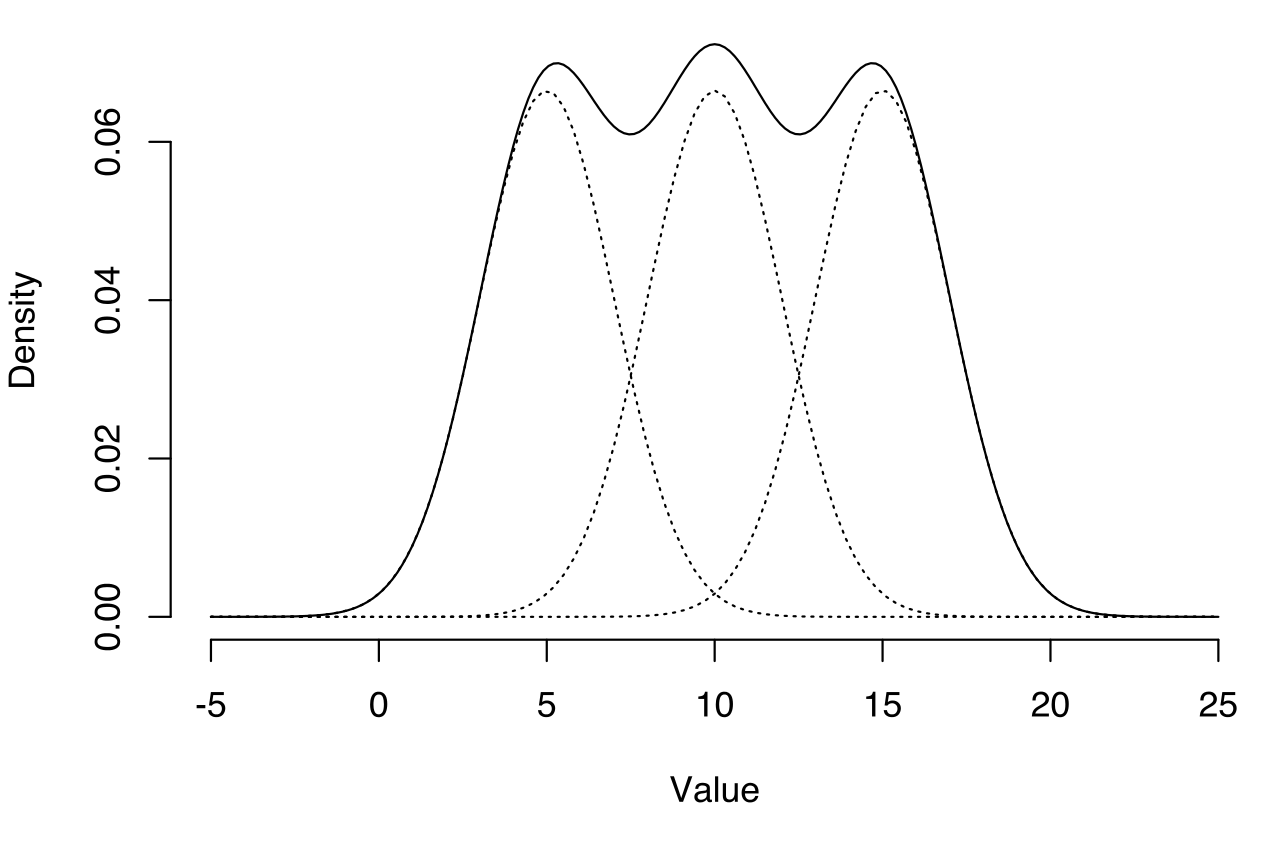
\includegraphics[width=0.6\textwidth]{fig/gaussian-mixture-distribution.png}
    \caption{混合分布}
    \label{fig:mix-dist}
\end{figure}

由于对数收益率的的可叠加性(较长时间内的对数收益率可分解为较短时间间隔对数收益率相叠加),并且利用上述正态分布性质,可知正态分布随机变量$d\ln S$(极短时间内)与叠加之后的$\Delta \ln S$(较长时间内)都应服从\textbf{正态分布}。

对比\textbf{比例收益率}在极短时间内(连续形式)与较长时间内(离散形式):
\begin{align*}
    \frac{dS_t}{S_t} &= \mu dt + \sigma dZ_t \\
    \frac{\Delta S_t}{S_t} &= \mu \Delta t + \sigma(Z_T - Z_t)
\end{align*}

百分比收益率虽然在极短时间(连续形式)服从正态分布。由于分母$S_t$不断改变,并不能通过叠加的形式得到较长时间的分布,即:
\begin{equation*}
    \frac{S_n - S_0}{S_0} \neq \frac{S_1- S_0}{S_0} + \frac{S_2-S_1}{S_1} + \dots + \frac{S_{n}-S_{n-1}}{S_{n-1}}
\end{equation*}

\textbf{存疑}:比例收益率在较短时间与较长时间应该也服从正态分布,通过累加两者服从的分布相同,变量不同,仅都服从同一正态分布。与对数收益率相比漂移项不同。且现实中比例收益率取值范围为$[-100\%,+\inf)$,并不符合正态分布,这点与模型不符。$\Delta S$则不服从正态分布,随着$S_t$的变化,其均值与方差也在不断改变。

\section{对数正态分布}

由\textbf{股票价格的对数}服从\textbf{正态分布}可知,股票价格应服从\textbf{对数正态分布}(Log-normal distribution)。由正态分布与对数正态分布的性质可知,对一个服从正态分布的随机变量$X$取指数,则$e^X$服从对数正态分布。相反,对一个服从对数正态分布的随机变量$X$取对数,则$\ln X$服从正态分布(因而得名,取对数得到正态分布的分布)。因此有如下关系:
\begin{align*}
    \ln S_T \sim N(\mu,\sigma^2) \quad \leftrightarrow \quad S_T \sim \text{Log-normal}(\mu,\sigma^2)
\end{align*}

已知对数正态分布$X \sim \text{Log-normal}(\mu,\sigma^2)$,其期望与标准差为:
\begin{align*}
    \E(X) & = e^{\mu+\frac{\sigma^2}{2}} \\
    \Var(X) & = e^{2\mu+\sigma^2} (e^{\sigma^2}-1)
\end{align*}

已知股票价格的对数$\ln S_T$服从如下正态分布:
\begin{equation*}
    \ln S_T  \sim N \left(\ln S_t + (\mu-\frac{\sigma^2}{2})(T-t), \sigma^2(T-t)\right)
\end{equation*}

可知股票价格$S_T$服从对数正态分布,代入上式可知其期望及方差为:
\begin{align*}
    \E(S_T)   & = \exp\left( \ln S_t + (\mu - \frac{\sigma^2}{2})(T-t)+\frac{\sigma^2(T-t)}{2}\right) \\
    & = \exp \left( \ln S_t + \mu(T-t) \right) \\
    & = S_t e^{\mu(T-t)} \\
    \Var(S_T) & = \left[\exp(\sigma^2(T-t))-1\right] \exp \left\{2\left[\ln S_t + (\mu - \frac{\sigma^2}{2})(T-t)\right] + \sigma^2(T-t)\right\} \\
    & = \left[\exp(\sigma^2(T-t))-1\right] \exp\left[2 \ln S_t + 2\mu (T-t)\right] \\
    & = S_t^2 e^{2\mu(T-t)} \left[ e^{\sigma^2 (T-t)} - 1 \right]
\end{align*}

\subsection*{注意}

对于正态分布$\mu$与$\sigma^2$,为其均值与标准差。而对于对数正态分布,仅为确定其分布的两个参数。对于相同的$\mu$与$\sigma$参数确定的正态分布与对数正态分布,两者之间的期望与方差通过如下表格关系转化:
\begin{table}[H]
\centering
\begin{tabular}{@{}cll@{}}
\toprule
\multicolumn{1}{l}{}
& \multicolumn{1}{c}{\textbf{正态分布}} & \multicolumn{1}{c}{\textbf{对数正态分布}} \\
\midrule
\multirow{1}{*}{\textbf{期望}} 
& $\E_N(X) \equiv \mu = \ln[\E_{L}(X)] - \frac{1}{2} \ln \left[1+\frac{\Var_{L}(X)}{[\E_{L}(X)]^2}\right] $ & $\E_{L}(X) = e^{\mu+\frac{1}{2}\sigma^2}$ \\
\textbf{方差} & $\Var_N(X) \equiv \sigma^2 = \ln \left[1+\frac{\Var_{L}(X)}{[\E_{L}(X)]^2}\right]$ & $\Var_{L}(X) = e^{2\mu+\sigma^2} 
\left(e^{\sigma^2} - 1\right)$ \\
\bottomrule
\end{tabular}
\end{table}

\subsection{PDF与CDF}

如下图所示,通过对服从\textbf{正态分布}的随机变量\textbf{取指数},可以将其转换为对数正态分布。同理,通过对服从\textbf{对数正态分布}的随机变量\textbf{取对数},使其转换为正态分布。假设随机变量$Y \sim N(\mu,\sigma^2)$ 服从正态分布,随机变量$X \sim \text{Log}N(\mu,\sigma^2)$,对正态分布随机变量$Y$取指数$x=e^y$,此时有$y = \ln x$,带入CDF中,可得到对数正态函数CDF。对两者求导,可得PDF函数。
\begin{table}[H]
\centering
\begin{tabular}{@{}cll@{}}
\toprule
\multicolumn{1}{l}{}
& \multicolumn{1}{c}{\textbf{正态分布}} & \multicolumn{1}{c}{\textbf{对数正态分布}} \\
\midrule
\multirow{1}{*}{\textbf{PDF}} 
& $\frac{1}{\sigma\sqrt{2\pi}} e^{-\frac{1}{2} \left( \frac{x-\mu}{\sigma} \right)^2 } $
& $\frac{1}{x\sigma\sqrt{2\pi}} e^{-\frac{1}{2} \left( \frac{\ln x-\mu}{\sigma} \right)^2 } $ \\
\textbf{CDF} 
& $\frac{1}{2} \left[1 + \text{erf}\left( \frac{x-\mu}{\sigma\sqrt{2}}\right) \right]$
& $\frac{1}{2} \left[1 + \text{erf}\left( \frac{\ln x-\mu}{\sigma\sqrt{2}}\right) \right]$ \\
\bottomrule
\end{tabular}
\end{table}

\begin{figure}[ht!]
    \centering
    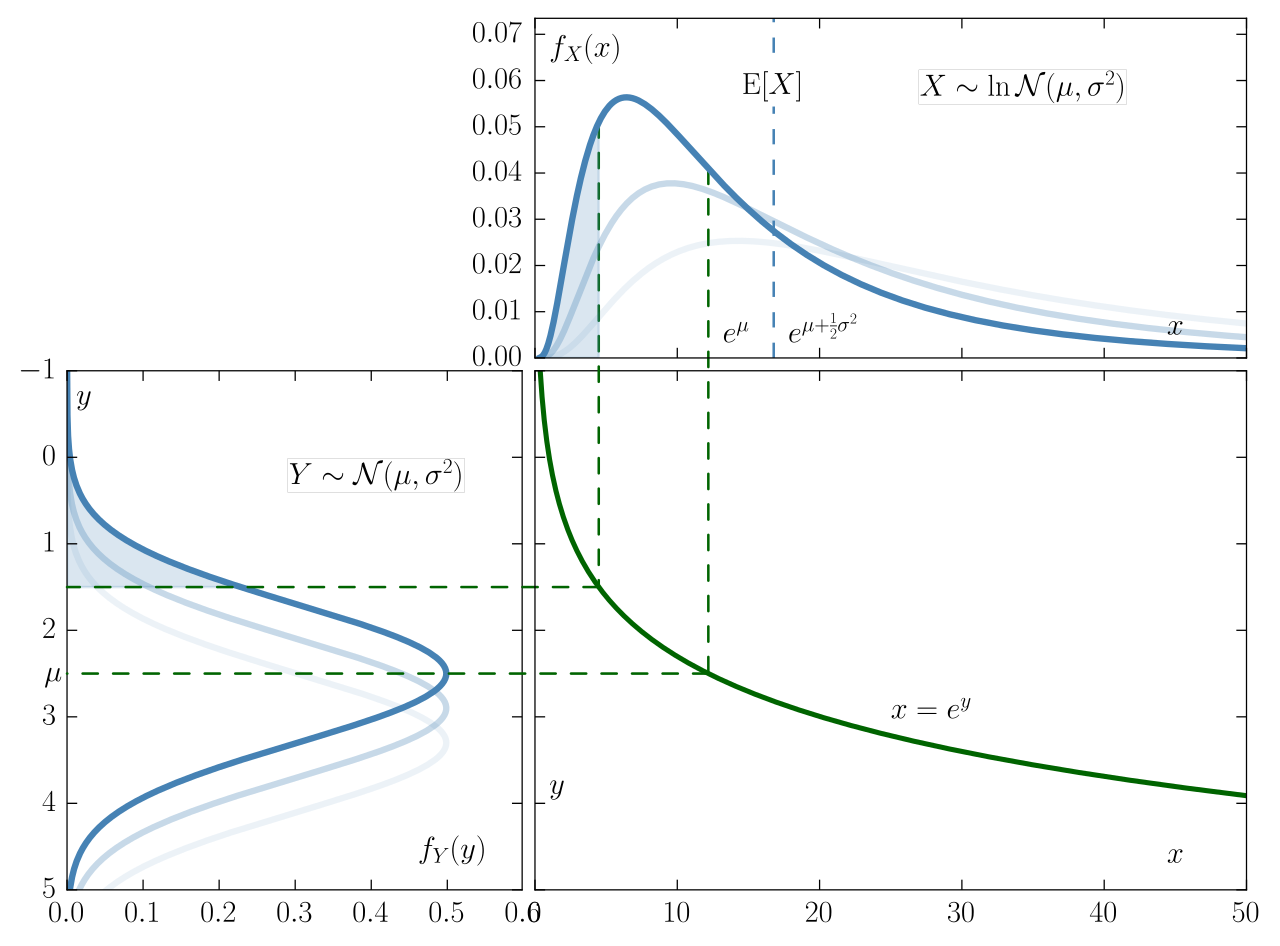
\includegraphics[width=0.9\textwidth]{fig/lognormal-distribution.png}
    \caption{两者相互转换}
    \label{fig:lognormal}
\end{figure}

\subsection{具体推导}

如上文所述,对于相同参数$\mu$与$\sigma^2$的正态分布与对数正态分布可以相互转化。两者互相经过转化后,其累积分布函数(Cumulative distribution fuction,CDF)相同。如图\ref{fig:lognormal}所示,假设随机变量$Y \sim N(\mu,\sigma^2)$ 服从正态分布,随机变量$X \sim \text{Log}N(\mu,\sigma^2)$,则应有如下关系,对服从对数正态分布的随机变量$X$取对数,使其转化为正态分布:
\begin{equation*}
    \text{CDF}_{logN}(x) = \text{CDF}_N (\ln x) = \text{CDF}_N (y)
\end{equation*}

对公式两边取导数,则可得到其概率密度函数(Probability density function,PDF):
\begin{equation*}
    \text{PDF}_{logN}(x) = \frac{1}{y} \text{PDF}_N(\ln x)
\end{equation*}

此时,带入已知正态分布PDF,即可得到对数正态分布PDF:
\begin{equation*}
    \text{PDF}_{logN} = \frac{1}{x\sigma\sqrt{2\pi}} e^{-\frac{(\ln x - \mu)^2}{2\sigma^2}}
\end{equation*}

\subsubsection{期望推导}

根据对数正态分布的PDF,可计算其期望:
\begin{equation*}
    \E(X) = \int^{+\infty}_0 x f(x) dx = \int^{+\infty}_0 \frac{1}{\sigma\sqrt{2\pi}} e^{-\frac{(ln x - \mu)^2}{2\sigma^2}} dx
\end{equation*}

使用换元法,令$t = \frac{\ln x - \mu}{\sqrt{2}\sigma}$,则有$x = e^{\sqrt{2}\sigma t + \mu}$,则原积分转化为:
\begin{align*}
    \E(X) &= \int^{+\infty}_{-\infty} \frac{1}{\sigma\sqrt{2\pi}}e^{-t^2}d e^{\sqrt{2}\sigma t + \mu}\\ 
    &= \frac{e^{\mu + \frac{\sigma^2}{2}}}{\sqrt{\pi}} \int^{+\infty}_{-\infty} e^{-(t-\frac{\sqrt{2}\sigma}{2})^2} dt\\ 
    &= \frac{e^{\mu + \frac{\sigma^2}{2}}}{\sqrt{\pi}} \int^{+\infty}_{-\infty} e^{-t^2}d e^{-(t-\frac{\sqrt{2}\sigma}{2})^2} d(t-\frac{\sqrt{2}\sigma}{2})
\end{align*}

由于$\int^{+\infty}_{-\infty} e^{x^2} = \sqrt{\pi}$,可得到:
\begin{equation*}
    \E(X) = e^{\mu+\frac{\sigma^2}{2}}
\end{equation*}

\subsubsection{方差推导}

已知:
\begin{equation*}
    \Var(X) = \E[(X-\mu)^2] = \E(X^2 -2\mu X + \mu^2) = \E(X^2) -2\mu \E(X) + \mu^{2} = \E(X^2) - [\E(X)]^2
\end{equation*}

同上,已知对数正态分布PDF:
\begin{equation*}
    \E(X^2) = \int^{+\infty}_0 x^2 f(x) dx = \int^{+\infty}_0 \frac{x}{\sigma\sqrt{2\pi}} e^{-\frac{(\ln x - \mu)^2}{2\sigma^2}} dx
\end{equation*}

使用换元法,令$t = \frac{\ln x-\mu}{\sigma}$,则有$x = e^{\sigma t + \mu}$:
\begin{align*}
    \E(X^2) &= \frac{e^{2\mu}}{\sqrt{2\pi}} \int^{+\infty }_{-\infty } e^{-\frac{t^2}{2}+2\sigma t}dt \\
    &= \frac{e^{2\mu}}{\sqrt{2\pi}} \int^{+\infty }_{-\infty } e^{-\frac{1}{2}(t-2\sigma)^2 + 2\sigma^2}dt \qquad 
    \left(\text{对}-\frac{t^2}{2}+2 \sigma t \text{配方}\right) \\
    &= \frac{e^{2\mu+2\sigma^2}}{\sqrt{2\pi}} \sqrt{2} \int^{+\infty}_{-\infty} e^{(-\frac{t-2\sigma}{\sqrt{2}})^2} d\left(\frac{t-2\sigma}{\sqrt{2}}\right)\\
    &= e^{2\mu +2\sigma^2}
\end{align*}

此时则有:
\begin{align*}
    \Var(X) &= \E(X^2) - [\E(X)]^2  \\
    &= e^{2\mu+2\sigma^2} - (e^{\mu+\frac{\sigma^2}{2}})^2 \\
    &= e^{2\mu+2\sigma^2} - e^{2\mu+\sigma^2} \\
    &= e^{2\mu+\sigma^2}\left(e^{\sigma^2} - 1\right)\\
\end{align*}

\section{BSM 偏微分方程(PDE)}

\subsection{假设}
\begin{itemize}
    \setlength{\itemsep}{0em}
    \item 人性假设
    \begin{itemize}
        \item 不存在无风险套利机会(无套利)
    \end{itemize}
    \item 完美世界
    \begin{itemize}
        \item 允许卖空标的证券
        \item 没有交易费用和税收
        \item 证券交易时连续的,价格变动也是连续的
        \item 所有证券都完全可分
    \end{itemize}
    \item 可交易资产
        \begin{itemize}
            \item 证券价格遵循几何布朗运动,即$\mu$和$\sigma$为常数
            \item 衍生品有效期内,无风险利率r为常数
            \item 衍生证券有效期内,标的证券没有现金收益支付
        \end{itemize}
\end{itemize}

\subsection{推导}

假设股票价格$S_t$遵循几何布朗运动,以及其离散形式有:
\begin{align*}
    d S_t & = \mu S_t dt + \sigma S_t d Z_t \\
    \Delta S_t & = \mu S_t \Delta t + \sigma S_t \Delta Z_t
\end{align*}

假设衍生品价格$f(S_t, t)$为$S_t$以及$t$的函数,根据伊藤引理可得其连续和离散形式有:

\begin{align*}
    df(S_t,t) & = \left(\frac{\partial f}{\partial S} \mu S_t  + \frac{\partial f}{\partial t} + \frac{1}{2}\frac{\partial^2 f}{\partial S^2} \sigma^2 S_t^2 \right)dt + \frac{\partial f}{\partial S} \sigma S_t dZ_t \\
    \Delta f(S_t,t) & = \left(\frac{\partial f}{\partial S} \mu S_t  + \frac{\partial f}{\partial t} + \frac{1}{2}\frac{\partial^2 f}{\partial S^2} \sigma^2 S_t^2 \right) \Delta t + \frac{\partial f}{\partial S} \sigma S_t \Delta Z_t
\end{align*}

由此可见,股票价格与衍生品价格的风险源均来自$\Delta Z_t$,因此可以构建投资组合,由一单位衍生品空头,以及$\partial f/\partial S$单位证券多头构成,进行对冲消除该风险源:
\begin{equation*}
    \Pi_t = -f_t + \frac{\partial f}{\partial S} S_t
\end{equation*}

在$\Delta t$时间内,该投资组合价值的变化$\Delta \Pi_t$来源其标的资产以及衍生品的价格变动,代入$\Delta S_t$与$\Delta f_t$可得:
\begin{align*}
    \Delta \Pi_t & = -\Delta f_t + \frac{\partial f}{\partial S} \Delta S_t \\
    & = -\left[ \left(\frac{\partial f}{\partial S} \mu S_t  + \frac{\partial f}{\partial t} + \frac{1}{2}\frac{\partial^2 f}{\partial S^2} \sigma^2 S_t^2 \right) \Delta t + \frac{\partial f}{\partial S} \sigma S_t \Delta Z_t \right] + \frac{\partial f}{\partial S} \left( \mu S_t \Delta t + \sigma S_t \Delta Z_t \right) \\
    & = -\left( \frac{\partial f}{\partial t} + \frac{1}{2}\frac{\partial^2 f}{\partial S^2} \sigma^2 S_t^2 \right) \Delta t \\
\end{align*}

由于此时组合消除了风险,因此组合只应获得无风险收益率:
\begin{align*}
    \Delta \Pi_t & = r \Pi_t \Delta t \\
    -\left( \frac{\partial f}{\partial t} + \frac{1}{2}\frac{\partial^2 f}{\partial S^2} \sigma^2 S_t^2 \right) \Delta t & =  r \left( -f_t + \frac{\partial f}{\partial S} S_t \right) \Delta t \\
\end{align*}

整理等式,消去$\Delta t$,即可得到\textbf{BSM偏微分方程}(Black-Scholes equation):
\begin{equation*}
    \frac{\partial f}{\partial t} + r S_t \frac{\partial f}{\partial S} + \frac{1}{2} \sigma^2 S_t^2 \frac{\partial^2 f}{\partial S^2} = r f_t
\end{equation*}

\section{BSM公式(鞅方法)}

在风险中性世界中,无收益资产在$t$时刻,其看涨期权价值的期望为:
\begin{equation*}
    \tilde{\E}_t \left[ \max(S_T-K,0) \right]
\end{equation*}

欧式看涨期权的现值应为其期望值以无风险利率进行贴现:
\begin{equation*}
    c = e^{-r(T-t)} \tilde{\E}_t \left[ \max(S_T-K,0) \right]
\end{equation*}

同时在风险中性世界下,漂移率$\mu$应等于无风险收益率r,因此有:
\begin{equation*}
    \ln S_T - \ln S_t \sim N \left((r-\frac{\sigma^2}{2})(T-t), \sigma^2(T-t)\right)
\end{equation*}

已知:
\begin{equation*}
    S_T = S_t \exp\left[\left(r-\frac{\sigma^2}{2}\right)\left(T-t\right) + \sigma\left(Z_T - Z_t \right)\right]
\end{equation*}

已知$Y = \frac{Z_T - Z_t}{\sqrt{T-t}} \sim N(0,1)$,其概率密度函数(PDF)为:
\begin{equation*}
    \varphi(y) = \frac{1}{\sqrt{2\pi}} e^{-\frac{1}{2}y^2}
\end{equation*}

在风险中性下的期望,可以改写为如下积分的形式:
\begin{align*}
    \tilde{\E}_t \left[ \max(S_T-K,0) \right] & = \tilde{\E}_t \left[ S_t e^{(r-\frac{1}{2}\sigma^2)(T-t) + \sigma\sqrt{T-t}Y} - K \right]^+ \\
    & = \int_{-\infty}^{\infty} \left( S_t e^{(r-\frac{1}{2}\sigma^2)(T-t) + \sigma\sqrt{T-t}y} - K \right)^+ \varphi(y) dy
\end{align*}

当$S_t e^{(r-\frac{1}{2}\sigma^2)(T-t) + \sigma\sqrt{T-t}Y} - K \geq 0$时,有$y \geq \frac{ \ln (K/S_t) - (r-\frac{1}{2}\sigma^2)(T-t)}{\sigma\sqrt{T-t}}$,设其为$-d_2$,同时假设$d_1 = d_2 + \sigma \sqrt{T-t}$。
\begin{align*}
    \tilde{\E}_t \left[ \max(S_T-K,0) \right] & = \int_{-\infty}^{\infty} \left( S_t e^{(r-\frac{1}{2}\sigma^2)(T-t) + \sigma\sqrt{T-t}y} - K \right)^+ \varphi(y) dy \\
    & = S_t e^{(r-\frac{1}{2}\sigma^2)(T-t)} \int_{-d_2}^{\infty} e^{\sigma\sqrt{T-t} y} \varphi(y)dy - K\int_{-d_2}^{\infty} \varphi(y)dy \\
    & = S_t e^{(r-\frac{1}{2} \sigma^2) (T-t)} \int_{-d_2}^{\infty}{e^{\sigma\sqrt{T-t}y} \frac{1}{\sqrt{2\pi\ }}e^{-\frac{y^2}{2}}dy} - KN\left(d_2\right) \\
    & = S_t e^{r(T-t)} \int_{-d_2}^{\infty} \frac{1}{\sqrt{2\pi}} e^{\left( -\frac{\sigma^2 (T-t)}{2} + \sigma\sqrt{T-t}y - \frac{y^2}{2} \right)} dy - KN(d_2) \\
    & = S_t e^{r(T-t)} \int_{y = -d_2}^{y = \infty} \frac{1}{\sqrt{2\pi}}e^{-\frac{\left(y-\sigma\sqrt{T-t}\right)^2}{2}}dy - KN(d_2) \quad \text{(换元法:$u =y -\sigma\sqrt{T-t}$)} \\
    & =S_t e^{r(T-t)} \int_{u = -d_2-\sigma\sqrt{T-t}}^{u = \infty} \frac{1}{\sqrt{2\pi\ }}e^{-\frac{u^2}{2}}du - KN(d_2) \quad \text{($dy = du$)} \\
    & = S_t e^{r(T-t)} \int_{-d_1}^{\infty} \frac{1}{\sqrt{2\pi}}e^{-\frac{u^2}{2}} du - KN(d_2) \\
    & = S_t e^{r(T-t)}N(d_1) - KN(d_2)
\end{align*}

得到\textbf{BSM公式}(Black-Scholes formula),即欧式看涨期权的解析解(注:$N(\cdot)$为标准正态分布的累积分布函数(CDF),而$N'(\cdot)$为标准正态分布的概率分布函数(PDF)):
\begin{align*}
    c & = e^{-r(T-t)} \tilde{\E}_t \left[ \max(S_T-K,0) \right] \\
    & = S_t N(d_1) - Ke^{-r(T-t)} N(d_2)
\end{align*}

已知期权平价公式:
\begin{equation*}
    c + K e^{r(T-t)} = p + S_t
\end{equation*}

代入BSM看涨期权解析解中,可得:
\begin{align*}
    p & = c + K e^{-r(T-t)} - S_t \\
    & = S_t N(d_1) - Ke^{-r(T-t)} N(d_2) +  Ke^{-r(T-t)} - S_t \\
    & = S_t (N(d_1) - 1) - K e^{-r(T-t)}(N(d_2)-1) \\
    & = S_t (-N(-d_1)) - K e^{-r(T-t)}(-N(-d_2)) \\
    & = K e^{-r(T-t)}N(-d_2) - S_t N(-d_1) \\
\end{align*}

此时$d_1$和$d_2$分别为:
\begin{align*}
    d_1 = \frac{\ln \frac{S_t}{K} + (r+\frac{1}{2}\sigma^2)(T-t)}{\sigma\sqrt{T-t}} \\
    d_2 = \frac{\ln \frac{S_t}{K} + (r-\frac{1}{2}\sigma^2)(T-t)}{\sigma\sqrt{T-t}}
\end{align*}

\section{波动率}

波动率为一种风险的度量,所有的计算方法都是一种近似估计,并不代表准确的波动率。波动率可以大致分为两类,一类为回望波动率(backward looking),一类为前瞻波动率(forward looking)。两者的区别在于回望波动率使用的是一段时间内的历史数据所计算出来的,是已经发生的波动率,如:历史波动率、已实现波动率、GARCH波动率。而后者为根据BSM模型等,根据期权市场现有的价格信息,倒求出其中所包含的波动率信息(隐含),为人们对未来给定期限的波动率的预期值,如:隐含波动率(包含无模型波动率)。

波动率的数学定义为:假设$r_t$为一个资产的收益率时间序列,有$t=1,2,3,\dots,T$,则有样本方差为:
\begin{equation*}
    \sigma^2(r_t) = \frac{1}{T-1} \sum^T_{t=1} (r_t - \bar{r})^2 
\end{equation*}

其中样本均值应有:
\begin{equation*}
    \bar{r} = \frac{1}{T} \sum_{t=1}^{T}r_t
\end{equation*}

\subsection{历史波动率(Historical volatility)}

样本对数收益率标准差(日频数据)

历史波动率,指资产收益率在过去一段时间内表现出的波动水平,可以由资产收益率在过去一段时间内的标准差计算得到。

TODO:关于 historical volatility。在 Black Scholes 的框架下,也就是假设股票价格服从 GBM 的时候,volatility 可以用 quadratic variation 计算。如下式:
\begin{equation*}
    \lim_{n\rightarrow \infty} \sum^{n}_{i=1}(X_{t_i} - X_{t_{i-1}})^2 = [X,X]_T = \sigma^2 T
\end{equation*}

其中$X_t$为股票价格的对数,$t_0,t_1,\dots,t_n$为$[0,T]$区间的一个划分。注意,这个和标准差不一样,这个其实是对数收益率的二阶距。可以证明,用 quadratic variation 得到的估计量是一致估计。

\subsection{已实现波动率(Readlized volatility)}

已实现波动率(Realized volatility,日内高频,5分钟,假设均值为零)

RV是瞬时或者高频的波动离散率,均值足够低,可用于预测或择时。打破了随机游走的假设。模拟了波动率的高聚集性。

参考Hansen和Lunde(2005),调整后的“已实现”波动率定义如下


\subsection{随机波动率(Sochastic volatility)}

随机波动率模型指随机过程的波动率为随机变量。
% https://en.wikipedia.org/wiki/Stochastic_volatility
\begin{itemize}
    \setlength{\itemsep}{0em}
    \item Heston model
    \item Constant elasticity of variance model  (CEV)
    \item SABR
    \item GARCH
\end{itemize}

\subsubsection{GARCH波动率}

GARCH为广义自回归条件异方差模型(Generalized autoregressive conditional heteroskedasticity)。Robert Engle于1982年在《计量经济学》上提出了ARCH模型用于估计和预测波动率。在此基础上,Bollerslev(1986)建立了广义自回归条件异方差(GARCH)模型。

\subsection{局部波动率(Local volatility)}

TODO: Local volatility,这个其实是一个作为 stochastic volatility 的一种替代做法,就是认为 volatility 是一个关于时间和资产价格的确定性函数$\sigma(t,S_t)$ ,因此也叫 Deterministic Volatility Function (DVF)。这样做也就是为了避免 Heston Model 等 stochastic volatility 带来的计算复杂度。Dupire 给出了一种计算 local volatility 的方法:
\begin{equation*}
    \sigma^2(K,T) = \frac{\frac{\partial C}{\partial T}}{\frac{1}{2} K^2 \frac{\partial^2 C}{\partial K^2}}
\end{equation*}


% https://en.wikipedia.org/wiki/Local_volatility

\subsection{隐含波动率(Implied volatility)}

\subsubsection{BS隐含波动率(BS implied volatility)}

假定市场上的期权或者权证的交易价格满足Black-Scholes-Merton(BSM)期权定价公式,将市场上可以观测到的标的资产价格($S$)、执行价格($K$)、利率($r$)、期限($\tau$)作为已知变量代入定价公式中,则可以得到期权当前的市场价格所隐含的波动率,此时提取的为期限内的波动率(Option-implied volatility expectations until expiration)。
\begin{align*}
    c &= S_t N(d_1) - Ke^{-r(T-t)} N(d_2) \\
    p & = K e^{-r(T-t)}N(-d_2) - S_t N(-d_1) \\
    d_1 &= \frac{\ln \frac{S_t}{K} + (r+\frac{1}{2}\sigma^2)(T-t)}{\sigma\sqrt{T-t}} \\
    d_2 &= \frac{\ln \frac{S_t}{K} + (r-\frac{1}{2}\sigma^2)(T-t)}{\sigma\sqrt{T-t}} = d_1 - \sigma\sqrt{T-t}
\end{align*}

\subsubsection{无模型波动率(Model-free implied volatility)}

\subsection{典型实证现象}

有些现象能够在几乎所有收益率的时间序列中观察到。一个好的条件异方差模型要能够捕捉大部分实证现象。在这个部分,我们列出在波动性分析中最知名典型实证现象。
% https://vinsight.shnyu.edu.cn/about_volatility.php

\subsubsection{波动率聚类}

如果 t−1时的波动率很高,t 时的波动率也很可能会很高。即,在 t−1 时的冲击不仅会增加 t−1 时的波动率,也会影响到 t 时的波动率。换句话说,市场在某些时期较为波动,在其他时间更为平静。波动率特征按照时间集中分类。GARCH 类模型能够很好地捕捉这一现象。事实上,这些模型更准确地来说,是衡量 t 时的波动率是如何依赖历史波动率 (和其他可能的条件变量)。

\subsubsection{肥尾现象}

收益率的时间序列通常呈现肥尾分布,又叫做超额峰度,或者尖峰。也就是说,它们的峰度(用方差的平方根标准化的第四中心矩)通常都大于3(高斯随机变量的峰度为3)。事实上,一种流行的检验高斯分布假设的方法,Jarque-Bera测试,能够同时测试此分布是否是对称的以及其峰度是否等于3。

如果收益率是肥尾分布的,则极端事件(非常高或非常低的回报率)的发生概率会高于收益率分布满足正态(高斯)分布时其发生的概率。

大部分波动率模型,例如GARCH 模型会造成收益率呈现肥尾分布,不管真正的潜在冲击是高斯分布还是肥尾分布。在估计时,我们通常假设潜在冲击服从高斯分布。在样本量很大时,即使真实分布不是高斯,模型通常也能给出合适的估计值。这些估计值为最大似然估计值,并且能够在相对宽松的限制条件下给出一致的估计。

\subsubsection{不对称性}

有一个普通 GARCH 模型不能捕捉的实证现象是 t−1 时刻的负面冲击比正面冲击对 t 时刻的方差有更强烈的影响。尽管如此, GARCH 模型能够很容易地调整扩充从而捕捉到这种不对称性。类似的例子有门限 GARCH (TGARCH)模型,, 不对称 GARCH (AGARCH)模型和指数 GARCH (EGARCH))模型。

这一不对称性过去被成为杠杆效应,因为增加的风险被认为是来自于负面冲击所引起杠杆的增加,但是限制人们认识到这个效应不能解释所有现象,并且风险规避是一个重要的机制。


\section{希腊值}

\subsection{正态分布与性质}

对于正态分布或高斯分布(Gaussian distribution),其\textbf{概率密度函数}(Probability Density Function,PDF):
\begin{equation*}
    f(x;\mu,\sigma) = \frac{1}{\sigma\sqrt{2\pi}} e^{-\frac{1}{2}\left(\frac{x-\mu}{\sigma} \right)^2}
\end{equation*}

则有$N(x)$为标准正态分布(Standard normal distribution)的\textbf{累积分布函数}(CDF,Cumulative Distribution Function)为:
\begin{equation*}
    N(x) = \frac{1}{\sqrt{2\pi}} \int_{-\infty}^{x}e^{-\frac{z^2}{2}}dz
\end{equation*}

则有$N'(x)$为标准正态分布的概率密度函数:
\begin{equation*}
    N'(x) = \frac{1}{\sqrt{2\pi}} e^{-\frac{x^2}{2}}
\end{equation*}

由于正态分布的对称性,易知:
\begin{equation*}
    N(-x) = 1-N(x) \qquad
    N'(x) = N'(-x)
\end{equation*}

\subsection{希腊值定义}

定义衍生品价格,对标的价格的一阶导为Delta,对标的价格的二阶导为Gamma,对于期限的一阶导为Theta,对于无风险利率的一阶导为Rho,对于波动率的一阶导为Sigma。
\begin{equation*}
    \text{Delta} = \frac{\partial V}{\partial S} \qquad 
    \text{Gamma}  = \frac{\partial^2 V}{\partial S^2} \qquad
    \text{Theta} = -\frac{\partial V}{\partial \tau} \qquad
    \text{Rho} = \frac{\partial V}{\partial r} \qquad
    \text{Vega} = \frac{\partial V}{\partial\sigma} \qquad
\end{equation*}

\subsection{Black模型}

\begin{align*}
    C &= e^{-r\tau}[FN(d_1) - KN(d_2)] \\
    P &= e^{-r\tau}[KN(-d_2) - FN(-d_1)]
\end{align*}

其中有:
\begin{align*}
    d_1 &= \frac{\ln(F/K) + \sigma^2/2\tau}{\sigma \sqrt{\tau}} \\
    d_2 &= \frac{\ln(F/K) + \sigma^2/2\tau}{\sigma \sqrt{\tau}} \\
    d_2 &= d_1 - \sigma \sqrt{\tau}
\end{align*}

\begin{equation*}
    \frac{\partial d_1}{\partial F} = \frac{\partial d_2}{\partial F} = \frac{\frac{\partial \ln(F/K)}{\partial F} \sigma \sqrt{\tau}}{(\sigma \sqrt{\tau})^2} = \frac{\partial (\ln F - \ln K)/\partial F}{\sigma\sqrt{\tau}} = \frac{1}{F\sigma\sqrt{\tau}}
\end{equation*}

\subsubsection{Delta}

\begin{align*}
    FN'(d_1) &= \frac{F}{\sqrt{2\pi}}e^{-d_1^2/2} \\
    KN'(d_2) &= \frac{K}{\sqrt{2\pi}}e^{-d_2^2/2} = \frac{K}{\sqrt{2\pi}}e^{-d_1^2/2+d_1\sigma\sqrt{\tau}-\sigma^2\tau/2} \\
    &= \frac{K}{\sqrt{2\pi}}e^{-d_1^2/2+\ln(F/K)} 
    \qquad \left(d_1\sigma\sqrt{\tau} = \ln(F/K)+\sigma^2\tau\right) \\
    &= \frac{F}{\sqrt{2\pi}}e^{-d_1^2/2} \\
    &= FN'(d_1) \\
    \text{Delta}_c &= e^{-r\tau}[N(d_1) + FN'(d_1)\frac{\partial d_1}{\partial F} - KN'(d_2)\frac{\partial d_2}{\partial F}] \\
    &= e^{-r\tau}N(d_1) \\
    \text{Delta}_p &= e^{-r\tau}[KN'(-d_2)\frac{\partial d_2}{\partial F} - N(-d_1) - FN'(-d_1)\frac{\partial d_1}{\partial F}] \\
    &= e^{-r\tau}(-N(-d_1)) \qquad \left(KN'(-d_2) = KN'(d_2),\, FN'(-d_1)= FN'(d_1)\right) \\
    &= e^{-r\tau}(N(d_1)-1)
\end{align*}

\subsection{BSM模型}

\begin{align*}
    C_t &= S_te^{-q\tau}N(d_1) - Ke^{-r\tau}N(d_2) \\
    P_t &= -S_te^{-q\tau}N(-d_1) + Ke^{-r\tau}N(-d_2)
\end{align*}

其中有:
\begin{align*}
    d_1 &= \frac{\ln(S/K) + (r+\frac{\sigma^2}{2})\tau}{\sigma \sqrt{\tau}} \\
    d_2 &= \frac{\ln(S/K) + (r-\frac{\sigma^2}{2})\tau}{\sigma \sqrt{\tau}} \\
    d_2 &= d_1 - \sigma \sqrt{\tau}
\end{align*}

\begin{lemma}
    \begin{equation*}
        \frac{\partial d_2}{\partial S} = \frac{\partial d_1}{\partial S} = \frac{\frac{\partial \ln(S/K)}{\partial S} \sigma \sqrt{\tau}}{(\sigma \sqrt{\tau})^2} = \frac{\partial (\ln S - \ln K)/\partial S}{\sigma\sqrt{\tau}} = \frac{1}{S\sigma\sqrt{\tau}}
    \end{equation*}
    \begin{equation*}
        \frac{\partial d_2}{\partial \tau} = \frac{\partial d_1}{\partial \tau} - \frac{1}{2}\frac{\sigma}{\sqrt{\tau}}
    \end{equation*}
    \begin{equation*}
        \frac{\partial d_2}{\partial \sigma} = \frac{\partial d_1}{\partial \tau} - \sqrt{\tau}
    \end{equation*}
    \begin{equation*}
        \frac{\partial d_2}{\partial r} = \frac{\partial d_1}{\partial r}
    \end{equation*}
\end{lemma}

\begin{lemma}
    对于BSM公式,有:
    \begin{equation*}
        S_t N'(d_1) = Ke^{-r\tau} N'(d_2)
    \end{equation*}
\end{lemma}

\begin{proof}
    已知:
    \begin{align*}
        d_2^2-d_1^2 &= (d_2-d_1)(d_2+d_1) \\
        &= (-\sigma\sqrt{\tau})(2d_1-\sigma\sqrt{\tau}) \\
        &= (-\sigma\sqrt{\tau})\left(\frac{2\ln(S_t/K) + 2(r+\sigma^2/2)\tau}{\sigma\sqrt{\tau}} -\sigma\sqrt{\tau}\right) \\
        &= -2\left[\ln\frac{S_t}{K}+r\tau\right]
    \end{align*}

    同时已知$N'(x)=\frac{1}{\sqrt{2\pi}} e^{-\frac{x^2}{2}}$,则有:
    \begin{equation*}
        \ln\left(\frac{N'(d_1)}{N'(d_2)}\right)
        = -\frac{d_1^2}{2} + \frac{d_2^2}{2}
        = \frac{1}{2} (d_2^2-d_1^2)
        = -\left[\ln\frac{S_t}{K} +r\tau\right]
    \end{equation*}

    对等式两边取指数:
    \begin{align*}
        \frac{N'(d_1)}{N'(d_2)} 
        &= \exp\left( -\left[\ln\frac{S_t}{K} +r\tau\right] \right) \\
        &= \exp \left( \ln\frac{K}{S_t}-r\tau \right) \\
        &= \frac{K}{S_t} e^{-r\tau} \\
        S_t N'(d_1) &= Ke^{-r\tau} N'(d_2)
    \end{align*}
\end{proof}

\subsubsection{Delta}

\noindent
\begin{align*}
    \text{Delta}_c &= \frac{\partial C}{\partial S}
    = N(d_1) + \frac{1}{S_t\sigma\sqrt{\tau}} \left[ S_t N'(d_1)-Ke^{-r\tau}N'(d_2) \right] = N(d_1) \\
    \text{Delta}_p &= \frac{\partial P}{\partial S}
    = -N(-d_1) + \frac{1}{S_t\sigma\sqrt{\tau}} \left[ S_t N'(d_1)-Ke^{-r\tau}N'(d_2) \right] = N(d_1)-1
\end{align*}

对于已知$\partial C/\partial S$,可对PCP求导:

\subsubsection{Gamma}

对于gamma而言,calls和puts相同
\begin{equation*}
    \text{Gamma} = \frac{\partial^2 V}{\partial S^2} = \frac{\partial N(d_1)}{\partial S} = N'(d_1)\frac{\partial d_1}{\partial S} = \frac{N'(d_1)}{S\sigma\sqrt{\tau}}
\end{equation*}

\subsubsection{Theta}

对于欧式看涨期权有:
\begin{equation*}
    \text{Theta}_c = \frac{\partial C}{\partial \tau} = -\frac{S_t N'(d_1)\sigma}{2\sqrt{\tau}} - r K e^{-r\tau}N(d_2)
\end{equation*}

证明:
\begin{align*}
    \text{Theta}_c &= -\frac{\partial C}{\partial \tau} = - \frac{\partial [S_t N(d_1) - Ke^{-r\tau} N(d_2)]}{\partial \tau} \\ 
    &= -\frac{\partial S_t N(d_1)}{\tau} + \frac{\partial Ke^{-r\tau} N(d_2)}{\partial \tau} \\ 
    &= -S_t N'(d_1)\frac{\partial d_1}{\partial \tau} - rKe^{-r\tau}N(d_2) + Ke^{-r\tau} N'(d_2)\frac{\partial d_2}{\partial \tau} \\
    &= -S_t N'(d_1)\frac{\partial d_1}{\partial \tau} - rKe^{-r\tau} N(d_2) + Ke^{-r\tau}N'(d_2)\left(\frac{\partial d_1}{\partial \tau} -\frac{1}{2}\frac{\sigma}{\sqrt{\tau}} \right) \\
    &= \frac{\partial d_1}{\partial \tau} \left[\cancel{-S_t N'(d_1) + Ke^{-r\tau} N'(d_2) } \right] + Ke^{-r\tau} \left[ -rN(d_2) -\frac{1}{2}\frac{\sigma}{\sqrt{\tau}} N'(d_2)\right] \\
    &=  -\frac{1}{2}\frac{\sigma}{\sqrt{\tau}}S_t N'(d_1) - rKe^{-r\tau} N(d_2)
\end{align*}

对于欧式看跌期权有:
\begin{equation*}
    \text{Theta}_p = \frac{\partial P}{\partial \tau} = -\frac{S_t N'(d_1)\sigma}{2\sqrt{\tau}} + r K e^{-r\tau}N(-d_2)
\end{equation*}

证明:
\begin{align*}
    \text{Theta}_p &= -\frac{\partial P}{\partial \tau} = - \frac{\partial [-S_t N(-d_1) + Ke^{-r\tau} N(-d_2)]}{\partial \tau} \\ 
    &= \frac{\partial S_t N(-d_1)}{\tau} - \frac{\partial Ke^{-r\tau} N(-d_2)}{\partial \tau} \\ 
    &= S_t N'(-d_1)\frac{\partial d_1}{\partial \tau} + rKe^{-r\tau}N(-d_2) - Ke^{-r\tau} N'(-d_2)\frac{\partial d_2}{\partial \tau} \\
    &= S_t N'(d_1)\frac{\partial d_1}{\partial \tau} + r Ke^{-r\tau} N(-d_2) - Ke^{-r\tau}N'(d_2)\left(\frac{\partial d_1}{\partial \tau} -\frac{1}{2}\frac{\sigma}{\sqrt{\tau}} \right) \\
    &= \frac{\partial d_1}{\partial \tau} \left[\cancel{S_t N'(d_1) - Ke^{-r\tau} N'(d_2) } \right] + Ke^{-r\tau} \left[ rN(-d_2) -\frac{1}{2}\frac{\sigma}{\sqrt{\tau}} N'(d_2)\right] \\
    &=  -\frac{1}{2}\frac{\sigma}{\sqrt{\tau}}S_t N'(d_1) + rKe^{-r\tau} N(-d_2) \\
    &=  -\frac{1}{2}\frac{\sigma}{\sqrt{\tau}}S_t N'(d_1) + rKe^{-r\tau}[1- N(d_2) ] = \text{Theta}_c + rKe^{-r\tau}
\end{align*}

另有,利用Put-Call Parity可知:
\begin{equation*}
    C + Ke^{-r\tau} = P + S_t \qquad \Rightarrow \qquad \frac{\partial C}{\partial \tau} - rKe^{-r\tau} = \frac{\partial P}{\partial \tau} 
\end{equation*}

等式两边对$\tau$求偏导:
\begin{align*}
    -\frac{\partial P}{\partial \tau} & = -\frac{\partial C}{\partial \tau} + rKe^{-r\tau} \\
    \text{Theta}_p &= \text{Theta}_c + rKe^{-r\tau} \\
\end{align*}

\subsubsection{Vega}

对于Vega而言,calls和puts相同
\begin{equation*}
    \text{Vega} = \frac{\partial V}{\partial \sigma}  = SN'(d_1)\sqrt{\tau}
\end{equation*}

推导:
\begin{align*}
    \text{Vega} &= \frac{\partial C}{\partial \sigma} = \frac{\partial}{\partial \sigma} \left[S N(d_1) - K e^{-r\tau}N(d_2)\right] \\
    &= S N'(d_1) \frac{\partial d_1}{\partial \sigma} - Ke^{-r\tau}N'(d_2) \frac{\partial d_2}{\partial \sigma} \\
    &= S N'(d_1) \frac{\partial d_1}{\partial \sigma} - Ke^{-r\tau}N'(d_2) \left[ \frac{\partial d_1}{\partial \sigma} -\sqrt{\tau} \right] \qquad \text{(对$d_2 = d_1 - \sigma\sqrt{\tau}$求导)} \\
    &= \left[ S N'(d_1) - Ke^{-r\tau}N'(d_2) \right] \frac{\partial d_1}{\partial \sigma} + Ke^{-r\tau}N'(d_2) \sqrt{\tau} \\
    &= S N'(d_1)\sqrt{\tau} \qquad \text{(已知$S N'(d_1) = Ke^{-r\tau}N'(d_2)$)}
\end{align*}


\section{Delta对冲}

Delta为衍生品价格变动与其标的资产价格变动的比率。如果假定股票价格(X)与期权价格(Y)为折线,则其斜率应为Delta,即对股票价格变动一单位,期权价格变动$\Delta$单位。而现实中并非折线,Delta则为两者切线斜率。
\begin{equation*}
    \Delta = \frac{\partial V}{\partial S}
\end{equation*}

而从持有标的资产和衍生品数量分别为$N_S$和$N_V$而言,为了维持对冲结果,易知对于每一单位标的资产,应使用$\Delta$单位衍生品进行对冲。
\begin{equation*}
    \Delta V \times N_V = \Delta S \times N_S \qquad \Rightarrow \qquad
    \Delta = \frac{\partial V}{\partial S} = \frac{N_S}{N_V}
\end{equation*}

如上所述,假定股票价格遵循几何布朗运动,则有在显示测度(Physical probability measure)下:
\begin{equation*}
    \frac{dS_t}{S_t} = \mu dt + \sigma dW_t
\end{equation*}

根据伊藤引理:
\begin{equation*}
    f(T,W_T) =f(t,W_t) = \int^T_t \frac{\partial f}{\partial u}du + \int^T_t \frac{\partial f}{\partial S} dW_t \frac{1}{2} + \int^T_t\frac{\partial ^2 f}{\partial S^2} 
\end{equation*}



在Bakshi and Kapadia 2003中,

在一段时间内的使用看涨看跌期权进行Delta对冲(\textbf{注意:}由几何布朗运动与伊藤过程推到而来,因此看涨看跌期权形式相同,买入看涨看跌期权,并卖出股票,净投资金额获得无风险收益)。
\begin{equation*}
    \text{Call Gain} = C_{t+\tau} - C_t - \Delta_t ( S_{t+\tau}-S_t) - \frac{r\tau}{365}(C_{t+\tau} - \Delta_t S_t)
\end{equation*}
\begin{equation*}
    \text{Put Gain} = P_{t+\tau} - P_t - \Delta_t ( S_{t+\tau}-S_t) - \frac{r\tau}{365}(P_{t+\tau} - \Delta_t S_t)
\end{equation*}

Long call, short delta stock/ short call, long delta stock

Long put, long delta stock/ short put, short delta stock

\section{平价期权}

当平值点为$S = K e^{-r(T-t)}$时,将其带入看涨BSM公式当中,则有:
\begin{equation}
    \frac{c}{S} = N(d_1) - N(d_2)
\end{equation}

对于看跌期权则有:
\begin{align*}
    \frac{p}{S} & = N(-d_2) - N(-d_1) \\
    & = 1 - N(d_2) - [1-N(d_1)] \\
    & = N(d_1) - N(d_2) = \frac{c}{S}
\end{align*}

对于$d_1$和$d_2$,此时有:
\begin{equation}
    d_1 = \frac{ln(S/K)+(r+\sigma^2/2)(T-t)}{\sigma\sqrt{T-t}} = \frac{\sigma}{2}\sqrt{T-t}
\end{equation}

\begin{equation}
    d_2 = \frac{ln(S/K)+(r-\sigma^2/2)(T-t)}{\sigma\sqrt{T-t}} = d_1 - \sigma\sqrt{T-t}= -\frac{\sigma}{2}\sqrt{T-t}
\end{equation}

则对于欧式平价期权:
\begin{align*}
    \frac{c}{S} & = \frac{p}{S} = N \left( \frac{\sigma\sqrt{T-t}}{2} \right) - N\left( -\frac{\sigma\sqrt{T-t}}{2} \right) \\
    & = 2N\left( \frac{\sigma\sqrt{T-t}}{2} \right) - 1 \\
    & = 2\left[\frac{1}{2} + \frac{1}{\sqrt{2\pi}} \left(\frac{\sigma\sqrt{T-t}}{2} - \frac{(\sigma\sqrt{T-t}/2)^3}{6} + \frac{(\sigma\sqrt{T-t}/2)^5}{40} - \dots + \dots\right) \right] - 1 \qquad (\text{使用泰勒展开}) \\
    & \approx \frac{\sigma\sqrt{T-t}}{2\pi} \approx 0.4\sqrt{T-t}
\end{align*}

\section{中国市场}

\subsection{内在价值}

由于:
\begin{equation*}
    \text{期权价值(Option value)} = \text{内在价值(Intrinsic value)} + \text{时间价值(Time value)}
\end{equation*}

内在价值为即\textbf{不考虑资产价格波动}的情况下,期权条款赋予期权多头的最高价值。而时间价值为\textbf{标的资产价格波动}为期权多头(权利方)所带来的隐含价值,由于期权权利方只有权力而无义务,因此期权的时间价值应该大于0。内在价值不受时间价值的影响,因而可以使用二分法。


若定义内在价值为,期权若在当下时点到期,期权所含的的价值(Hull,CME)。这样考虑的缺点为没有考虑货币的时间价值,且在中国市场由于现货的卖空限制,其价格高于其真实价格。
\begin{align*}
    \text{看涨期权内在价值} & = \max(S_t-K) \\
    \text{看跌期权内在价值} & = \max(K-S_t)
\end{align*}

在考虑货币时间价值的情形内在价值如下,缺点为依然没有考虑中国市场的卖空限制。
\begin{align*}
    \text{看涨期权内在价值} & = \max(S_t-Ke^{-r(T-t)}) \\
    \text{看跌期权内在价值} & = \max(Ke^{-r(T-t)}-S_t)
\end{align*}

因此考虑使用期货价格代替现货价格,以为期货市场多空双方均能自由表达其看法,因此有:
\begin{align*}
    \text{看涨期权内在价值} & = \max((F_{t,T}-K)e^{-r(T-t)}) \\
    \text{看跌期权内在价值} & = \max((K-F_{t,T})e^{-r(T-t)})
\end{align*}

由于在中国市场ETF期权有红利保护机制,即会下调行权价格,放大每手期权数量,相当于变相抬高了股票价格,或复权(加挂A标记的期权)。且在ETF中的成分股分红,其分红留在ETF当中。而ETF没有期货,只有股指期货,而股指期货不对分红进行调整,即没有红利保护,即其成分股分红后股指自然下跌。因而在使用股指期货或期权以及ETF现货或期权时,需要做红利调整。即在ETF现货中将红利剔除,此时有:
\begin{equation*}
    F_{t,T} = (S_t-I)e^{r(T-t)}
\end{equation*}

此时则有,将上式代入,在中国市场中:
\begin{align*}
    \text{看涨期权内在价值} & = \max((F_{t,T}-K)e^{-r(T-t)}+I) \\
    \text{看跌期权内在价值} & = \max((K-F_{t,T})e^{-r(T-t)}-I)
\end{align*}

因为平值点为使内在价值为零,则平值点定义为为$F_{t,T}=K$,这样定义使得实值虚值部分左右较为对称,有利于比较。此时有当$F<K$为OTM,此时值域为正,当$F>K$为ITM,则有值域为负。此时有对数在值状态(log-moneyness):
\begin{equation*}
    \ln{\frac{K}{K_{atm}}} = \ln{\frac{K}{F}}
\end{equation*}

同时可以发现,在PCP下:
\begin{equation*}
    c = p + (F_{t,T}-K) e^{-r(T-t)}
\end{equation*}

对于平直期权ATM,则有$F_{t,T}=K$,易得此时$c=p$。而当看涨期权为ITM,其内在价值部分不为零。而对于此时得看跌期权为OTM,其内在价值为零,而仅有时间价值,因此可以得到,在新平值点定义下的,相同行权价,相同期限的看涨看跌期权:
\begin{equation*}
    c_{\text{时间价值}} = p_{\text{时间价值}}
\end{equation*}

\subsection{做空限制}

且在中国市场中现货存在较大的做空限制,即在现货市场的价格由看多者和少量看空者决定,并不能反应所有投资者的真实情绪,以至于难以复制期权,违法BSM公式假设条件。解决方法有:
\begin{enumerate}
    \setlength{\itemsep}{0em}
    \item 使用期货进行贴现,得到其隐含现货价格,使用BSM进行计算,其中有:
    \begin{itemize}
        \item 期货隐含现货价格
        \begin{equation*}
            S^* = F e^{-q(T-t)}
        \end{equation*}
        \item 期权隐含现货价格
        \begin{equation*}
            S^* = (c-p) + Ke^{-r(T-t)}
        \end{equation*}
    \end{itemize}
    \item 直接使用Black公式,使用期货价格进行计算,即:
    \begin{equation*}
        c = e^{-r(T-t)} \left[ F_t N(d_1)-K N(d_2) \right]
    \end{equation*}
\end{enumerate}

\end{document}